
\chapter{Preliminaries}

Mathematics originated in \emph{reasoning} about number and geometry. Within
mathematics, the calculus is a subject involving the idea of an arbitrarily
small quantity.  We approach the calculus first by reviewing some aspects of
reasoning. Then we reason about the \emph{set}, which can provide a basis for
mathematical thought.  At the end of the chapter, we reason about the
\emph{function}, which plays a central role in the calculus.

\section{Reasoning}

In mathematics, every important result can be expressed as an
\emph{implication}.  The \emph{mind} may \emph{prove} an implication.  A deep
discussion of the mind is beyond our scope, but we shall discuss three crucial
acts of the human mind.  These acts culminate in reasoning, which allows the
proof of an implication.

The ability of the human mind to reason can be viewed as evidence for the
mind's having an immaterial aspect.\footnote{%
   In fact, each of the mind's three acts that we discuss in the text can on
   its own be taken as requiring the mind's immateriality.
}
\emph{Materialism} is the philosophical position according to which everything
that exists is matter.  Modern science describes the world just as consisting
of
\begin{itemize}
   \item bits of matter,
   \item the space through which they move, and
   \item the forces by which they interact.
\end{itemize}
So \emph{scientism}, according to which everything that exists can be
understood in terms of science, is the modern form of materialism.  Because
materialism is a popular position,\footnote{%
   Scientism is popular because of the lack of appreciation for (a) the God of
   classical theism and (b) the qualitative distinction between the scientist
   and what the scientist studies, between the observer and the observed,
   between the subject and the object.

   (a) Modern scientific theory allows one reasonably to imagine how any
   ordinary physical thing could come to be without divine interference in the
   natural order. Both classical theism and modern atheism oppose the idea of
   explaining ordinary things by way of divine interference.  Even if all gaps
   in the natural explanation of ordinary things were closed, then only the
   gods of pantheism would be eliminated. The God of classical theism would not
   thus be eliminated.  According to classical theism, logic requires God as
   the primary cause. The natural, ordinary causes which science explores are
   secondary causes. The primary cause is the cause of the secondary causes.
   
   (b) Beyond the secondary causes that science can explore are not only God's
   primary causality but also aspects of the explorer, the human person. While
   the human body might be the product of a natural process of evolution
   stretching over billions of years, the free will and the acts of the mind
   cannot even in principle be described in terms of science. Also, if
   subjective experience be real, then there is the problem of accounting for
   the subjective.  A perfect scientific description of the human brain, its
   interface to the ear, the properties of the concert hall in which the body
   sits, and the properties of a grand piano could never allow a deaf person to
   know the experience of hearing the pitch of Concert~A on the piano.  Science
   will always fail to capture some aspect of subjective experience. If
   subjective experience be real, then the scientist is not entirely scrutable
   in terms of science.

   The defender of scientism will not be impressed with these observations and
   will have answers that in turn do not impress the classical theist. The
   point here is that scientism is not a part of modern science, and modern
   science does not imply scientism.
}
the claim of the mind's immateriality is controversial.  Below we discuss, as
an example of reasoning, Roger Penrose's argument according to which either
\begin{enumerate}
   \item certain behaviors of the brain cannot be described by quantum
      mechanics and general relativity, or else
   \item the mind is not merely the physical brain.
\end{enumerate}
Penrose himself is a materialist and therefore thinks that modern physics fails
to describe the brain. After all, on Penroses's understanding, one who holds
that modern physics \emph{does} well describe the brain must conclude that the
mind is not merely the physical brain. Our purpose here is not to assert the
truth of Penrose's view, and we do not claim to demonstrate that materialism is
false. We do however claim that materialism is a philosophical choice that is
required neither by modern science nor by reason.

Merely to provide an interesting example of an argument, we shall look in more
detail at Penrose's thesis below, first when we consider what an implication is
and then, after we introduce the three acts of the mind, when we discuss the
proof of an implication.

\subsection{Logic}

A \emph{proposition} is a statement proposed as a truth. The proposition might
be either true or false, but it represents a claim about what is true. For
example, ``the sky is cloudy'' is a proposition. Below we shall consider the
mind's role in determining whether a proposition be true.

\subsection{Implication and Contrapositive Expression}

\begin{figure}
   \begin{center}
      \begin{framed}
         \begin{eqnarray*}
            2 + x = 7 &\Rightarrow& x = 5\\
            x \neq 5  &\Rightarrow& 2 + x \neq 7\\
         \end{eqnarray*}
      \end{framed}
   \end{center}
   \caption{The positive expression of an implication (top) and its
      contrapositive expression (bottom). In this example, $2 + x = 7$ is the
      hypothesis of the implication, and $x = 5$ is the conclusion. An
      implication is the assertion that if the hypothesis be true, then the
      conclusion must be true. The contrapositive expression of the implication
      is the assertion that if the conclusion be false, then the hypothesis
      must be false.
   }
\label{fig:contrapositive}
\end{figure}

An implication has the form of a conditional, ``if $H$, then $C$'', where each
of $H$ and $C$ stands for a proposition.  An implication is written compactly
in the form, ``$H \Rightarrow C$'' and can be read, ``$H$ implies $C$''.  Each
of the \emph{hypothesis} $H$ and the \emph{conclusion} $C$ stands for a
statement that could be either true or false, but $H \Rightarrow C$ is the
claim that $C$ must be true when $H$ be true, that $H$ is a sufficient
condition for $C$. Also, $H \Rightarrow C$ is equivalent to its
\emph{contrapositive} expression, that $C$ is a necessary condition for $H$, or
$[\lnot C] \Rightarrow [\lnot H]$, where the symbol ``$\lnot$'' means ``not''.
That is, $H$ is false when $C$ be false. See Figure~\ref{fig:contrapositive}.
For an implication, a true hypothesis implies a true conclusion, and a false
conclusion implies a false hypothesis.

Consider, for example, the Pythagorean Theorem. A theorem might not always be
written in the form of an implication, but a theorem can always be rewritten as
an implication. In it usual form, the Pythagorean Theorem is the claim that for
a right triangle the square of the length of the hypotenuse is equal to the sum
of (1) the square of the length of one side and (2) the square of the length of
the other side.  Here is the Pythagorean Theorem as an implication: If $a$ be
the length of one leg of a right triangle, and $b$ be the length of the other
leg, then the length of the hypotenuse is $\sqrt{a^2 + b^2}$.
\begin{figure}
   \begin{center}
      \begin{tikzpicture}
         \pgfmathsetmacro{\a}{3}
         \pgfmathsetmacro{\rs}{2}
         \pgfmathsetmacro{\rl}{4.5}
         \pgfmathsetmacro{\as}{asin(\a/2/\rs)}
         \pgfmathsetmacro{\al}{asin(\a/2/\rl)}
         \pgfmathsetmacro{\xs}{-\rs*cos(2*\as)}
         \pgfmathsetmacro{\ys}{+\rs*sin(2*\as)}
         \pgfmathsetmacro{\xl}{-\rl*cos(2*\al)}
         \pgfmathsetmacro{\yl}{+\rl*sin(2*\al)}
         \definecolor{ca}{hsb}{0.00,1.00,1.00}
         \definecolor{cb}{hsb}{0.33,1.00,0.70}
         \definecolor{cbp}{hsb}{0.33,1.00,0.40}
         \definecolor{cc}{hsb}{0.67,0.70,1.00}
         \definecolor{ccp}{hsb}{0.67,1.00,0.70}
         \draw [cc,thick] (0,0) -- ({2*\rs},0);
         \draw [cc] (\rs,0) node[anchor=north] {$c$};
         \draw [cc] (0,-0.1) -- (0,-0.3);
         \draw [cc] ({2*\rs},-0.1) -- ({2*\rs},-0.3);
         \draw [cc,<-] (0,-0.2) -- ({\rs-0.2},-0.2);
         \draw [cc,->] ({\rs+0.2},-0.2) -- ({2*\rs},-0.2);
         \draw [ccp,thick] ({2*\rs},0) -- ({2*\rl},0);
         \draw [ccp] (\rl,-0.2) node[anchor=north] {$c'$};
         \draw [ccp] (0,-0.4) -- (0,-0.6);
         \draw [ccp] ({2*\rl},-0.4) -- ({2*\rl},-0.6);
         \draw [ccp,<-] (0,-0.5) -- ({\rl-0.2},-0.5);
         \draw [ccp,->] ({\rl+0.2},-0.5) -- ({2*\rl},-0.5);
         \draw [gray,thin,domain=25:90] plot ({\a*cos(\x)},{\a*sin(\x)});
         \draw [ca,thick] (0,0) -- ({\rs+\xs},\ys);
         \draw [ca] ({0.5*(\rs+\xs)},{0.5*\ys}) node[anchor=north west]
         {$a$};
         \draw [cb,thick] ({\rs+\xs},\ys) -- ({2*\rs},0);
         \draw [cb] ({0.5*(3*\rs+\xs)},{0.5*\ys}) node[anchor=north east]
         {$b$};
         \draw [ca,thick] (0,0) -- ({\rl+\xl},\yl);
         \draw [ca] ({0.5*(\rl+\xl)},{0.5*\yl}) node[anchor=south east] {$a$};
         \draw [cbp,thick] ({\rl+\xl},\yl) -- ({2*\rl},0);
         \draw [cbp] ({0.5*(3*\rl+\xl)},{0.5*\yl}) node[anchor=south west]
         {$b'$};
      \end{tikzpicture}
   \end{center}
   \caption{Contrapositive expression of the Pythagorean Theorem. If the
      hypotenuse of a right triangle have some length other than $c = \sqrt{a^2
      + b^2}$, then the triangle cannot have both a leg of length $a$ and a leg
      of length $b$. In the figure, one regards first a right triangle that
      does have length $c$ for its hypotenuse. By extending the hypotenuse to a
      length $c'$ larger than $c$ but holding one leg's length fixed at $a$,
      one finds that the other leg's length must grow to a length $b'$ larger
      than $b$.  Similar reasoning applies to the shortening of the
      hypotenuse.%
   }
\label{fig:right-triangle}
\end{figure}
Here is the contrapositive expression of the same theorem: If the length of a
right triangle's hypotenuse be not $\sqrt{a^2 + b^2}$, then it is not the case
that both $a$ is the length of one leg, and $b$ is the length of the other leg.
See Figure~\ref{fig:right-triangle}.

Consider, for another example, Penrose's Thesis: If the human brain operate
according to general relativity and quantum mechanics, then the human brain is
not the human mind.  Here is the contrapositive expression: If the human brain
be the human mind, then the human brain does not operate according to general
relativity and quantum mechanics.

\begin{exercise}
   Invent two implications. For each implication, identify the hypothesis and
   the conclusion. Write each implication in its contrapositive expression.
\end{exercise}

In mathematics, an implication that is widely useful is a \emph{theorem}. An
implication of limited use, typically as an intermediate step in the proof of a
theorem, is a \emph{lemma}. Proving an implication involves the construction of
a sequence of \emph{valid arguments} that, taken together, are equivalent to
the implication.  The importance of the contrapositive expression lies in its
utility in a proof: Sometimes, proving an implication's contrapositive
expression is easier than proving the positive expression.  In any event,
proving an implication is the essence of reasoning, which produces useful
results in mathematics.

\subsection{Proof}

One must, in order to prove an implication, be able to grasp the meaning of
each term mentioned in a proposition, to judge the proposed relationships among
the terms, and to gather relevant propositions together in the right order to
form a judgment about another proposition.  St.~Thomas Aquinas identifies these
as the three acts of the mind.
\begin{enumerate}
   \item The mind \emph{simply apprehends} the concept behind a word or a
      phrase.\footnote{%
         Coppens, {\it A Brief Text-Book of Logic and Mental Philosophy},
         Chapter I, Article I\@: ``9. \emph{Simple apprehension} is the act of
         perceiving an object intellectually, without affirming or denying
         anything concerning it\ldots. The mind cannot take an object
         physically into itself; but it knows an object by taking it in
         intellectually, in a manner suited to its own nature; forming to
         itself an intellectual image\ldots.  The act of forming this mental
         image is called a \emph{conception}, and the fruit of it, the image
         itself, is the \emph{concept}, \emph{idea}, or \emph{notion} of the
         object.  The word `simple' added to apprehension emphasizes the fact
         that the apprehension neither affirms nor denies the existence of the
         object\ldots.  10. This intellectual image should not be confounded
         with the sensible image, or \emph{phantasm}, which is a material
         representation of material objects, and which is formed by the
         imagination, by means of the material organ of the brain\ldots.  For
         instance, I intellectually \emph{conceive} a triangle by apprehending
         a figure enclosed by three lines and thus having three angles. My
         notion or idea contains this and nothing more; it is very precise, and
         every one who conceives a triangle conceives it exactly the same way.
         But when I \emph{imagine} a triangle, I cannot help imagining it with
         sensible material accidents, as being of such or such a size and
         shape, a foot long at one time, a mile long at another. The picture
         may be vague, various pictures of triangles may be blended together;
         but it can never be universal, representing all possible triangles, as
         my idea does\ldots.''%
      }
   \item The mind \emph{judges} whether the two ideas connected by a
      proposition (like ``modesty is praiseworthy'') ought so to be
      connected.\footnote{%
         Coppens, Chapter I, Article III\@: ``17. A \emph{judgment} may be
         defined as `an act of the mind affirming or denying the agreement of
         two objective ideas'.  The mind in judging compares two ideas \ldots\
         and affirms or denies that they agree with one another; e.g., `modesty
         is praiseworthy'\ldots.  [If] the agreement or disagreement [be] seen
         to exist by the mere consideration or analysis of the ideas compared,
         the judgment is \emph{analytic}; it is also styled \emph{a priori},
         i.e., formed antecedently to experience\ldots. But if the agreement or
         disagreement [be] discovered consequently on experience, e.g., `gold
         is malleable', the judgment receives the opposite appellations of
         \emph{synthetic} [or] \emph{a posteriori}\ldots.  18.  If a judgment
         of either kind [be] arrived at by reasoning, it is \emph{mediately
         evident}; if the agreement or disagreement [be] seen without the aid
         of reasoning, the judgment is \emph{immediately evident}. That `ice is
         cold', is an immediate a posteriori judgment; that `there is nothing
         without a reason for it', is immediately known a priori; that `the sum
         of the angles of a triangle is equal to two right angles', is known
         mediately a priori; the physical laws are known mediately a
         posteriori.  19. A judgment expressed in words is called a
         \emph{proposition}.  The subject and predicate together are its
         \emph{matter}, and the affirmation or negation its \emph{form}; the
         \emph{copula} is always the verb `to be' in the present indicative,
         expressed or implied: `I see' is equivalent to `I am seeing', `He
         said' to `He is one who said', etc.''%
      }
   \item The mind \emph{reasons} to derive some of its judgments from other
      judgments.\footnote{%
         Coppens, Chapter II\@: ``22. \emph{Reasoning} is the mental act or
         process of deriving judgments, called conclusions, from other
         judgments, called premises.  The principle underlying all valid
         reasoning is that the conclusion is implicitly contained in the
         premises; therefore whoever grants the truth of the premises thereby
         really grants the truth of the conclusion.''%
      }
\end{enumerate}
In its third act, which operates on products of the other two acts, the mind
reasons by arranging propositions into an valid argument.

An \emph{argument} is a set of two or more propositions, one of which is the
\emph{conclusion} and the rest of which are \emph{premises}.  The mind may
judge an argument by comparing (a) the claims made in the premises, taken
together as though they were a single proposition, with (b) the claim made in
the conclusion.  If the meaning of the conclusion be contained in the premises,
then the argument is \emph{valid}; otherwise, it is \emph{invalid}.  Every
argument purports to be an implication whose hypothesis comprises the premises.

For example: If every man be mortal, and Socrates be a man, then Socrates is
mortal.
\begin{figure}
   \begin{center}
      \begin{framed}
         \begin{tabular}{l}
            Every man is mortal.\\
            Socrates is a man.\\
            \midrule
            Socrates is mortal.
         \end{tabular}
      \end{framed}
   \end{center}
   \caption{A valid argument.  The premises lie above the line, and the
      conclusion lies below the line.  If the premises be true, then the
      conclusion must be true.%
   }
\label{fig:valid-arg}
\end{figure}
This bit of reasoning is expressed in Figure~\ref{fig:valid-arg}.  In comparing
the premises to the conclusion, one recognizes the argument as valid.  Every
valid argument is obviously an implication.

Even if an argument's conclusion be not contained in the hypothesis, and so
long as the argument contain no contradiction, then something additional might
be provided in order for one to grasp that the argument is an implication.
What might be provided is a chain of arguments, each of which can be recognized
as valid, such that the chain is equivalent to the purported implication. The
first valid argument in the chain has among its premises the hypothesis of the
implication under examination, plus zero or more true statements brought in as
necessary.  The conclusion of that first valid argument then serves as a
premise for the next valid argument in the chain. That valid argument may
itself bring in additionally zero or more true statements as premises. This is
repeated as necessary. The conclusion of the final valid argument in the chain
is the conclusion of the implication under examination.

As an example, let us consider Penrose's thesis in some detail.
\begin{figure}
   \begin{center}
      \begin{framed}
         \begin{tabular}{p{0.9\columnwidth}}
            The human brain operates according to QM and GR.\\
            \midrule
            The human brain is not the human mind.
         \end{tabular}
      \end{framed}
   \end{center}
   \caption{An invalid argument that might still be an implication. `QM' stands
      for `quantum mechanics', and `GR' stands for `general relativity'.%
   }
\label{fig:brain}
\end{figure}
Figure~\ref{fig:brain} shows the initial argument.
\begin{figure}
   \begin{center}
      \begin{framed}
         \begin{tabular}{p{0.9\columnwidth}}
            The human brain operates according to QM and GR.\\
            QM and GR provide an algorithmic description.\\
            \midrule
            The human brain operates according to an algorithm.\\
            No algorithm can do math like the human mind. (G\"odel)\\
            \midrule
            The human brain is not the human mind.
         \end{tabular}
      \end{framed}
   \end{center}
   \caption{A chain of two valid arguments that Penrose uses to establish that
      the argument in Figure~\ref{fig:brain} is an implication.  The conclusion
      of the first is one of the premises of the second.  The second premise of
      the second argument refers to the Incompleteness Theorem of Kurt
      G\"odel.%
   }
\label{fig:brain2}
\end{figure}
Figure~\ref{fig:brain2} shows a summary of Penrose's proof.  There are two
valid arguments in the chain of reasoning. The first takes the original
hypothesis and adds a premise about the algorithmic nature of quantum mechanics
and general relativity. The first conclusion is then combined with the
Incompleteness Theorem of G\"odel in order to form a valid argument whose
conclusion is the same as the conclusion of the implication under examination.
In a proof, any new premises brought in must be true.  So an opponent of
Penrose might try to attack each of the two new premises as not being true, but
Penrose does seem to have provided deductively valid arguments in his chain.  A
chain of valid arguments is thus advanced to prove that the argument is an
implication.

The conclusion of an implication that has been proved is \emph{deduced} from
the premises. A deduction is certain to be true if the premises be true.

The conclusion of an argument that is not an implication is \emph{induced} from
the premises. An induction is not certain to be true even if the premises be
true. The \emph{problem of induction}, for a given set of true premises, is to
determine the probability of the conclusion's being true.  An argument has an
inductive strength proportional to the probability of its conclusion's truth,
given the truth of the premises.

The word ``sound'' when applied to an argument indicates both that the argument
is valid and that the premises are true.\footnote{%
   The root ``sund'' in the German word ``gesund'', which in English means
   ``healthy'', derives from the same root as does one of the English words
   spelled as ``sound''. There is more than one English word with the same
   spelling. A sound that one hears is not related to ``gesund'', but a sound
   argument is indeed properly a healthy argument.%
}
One of the problems with reasoning is that it cannot operate in a vacuum. While
the hypothesis of an implication might be the conclusion of another
implication, any line of reasoning can be traced back to a point at which at
least one premise is not itself the result of reasoning. So every application
of reasoning depends ultimately on some truths that are known independently of
any reasoning.  We can know some truths directly by the second act of the mind,
and the soundness of an argument must depend upon truths of that kind.

While a theorem in mathematics is a strict and certain implication, a theory in
modern science is not. A scientific theory involves, in its chain of reasoning,
one or more strong but invalid arguments. The Pythagorean Theorem takes the
lengths of the legs and concludes that the length of the hypotenuse is a
definite and certain value. However, even if the Sun is risen every morning
since the beginning of history, the conclusion that the Sun will rise again
tomorrow morning is \emph{not} certainly true.  The conclusion of the
Pythagorean Theorem is a deduction, but the claim about the Sun is, of its
scientific nature, a particular kind of induction taking the form of a
prediction about what will be observed with the senses.  A mathematical theorem
may be proved true, but a scientific theory can \emph{never} be proved true;
there is always the chance that eventually a bit of evidence ruling out the
scientific theory will turn up.

There is still a sense of proof in modern science, though. When a repeatable
observation be inconsistent with the prediction of a scientific theory, the
theory is proved false. After it has been ruled out by observation, the theory
is no longer a candidate for a true description of the physical world. The
theory may remain useful for engineering, but the theory has been shown
inconsistent with what is known directly through sense experience. Modern
science progresses by experimental proof of the \emph{lack} of implication in
the assertion of a scientific theory. Such progress ensures plenty of work for
theorists, who must come up with new theories as the old ones are ruled out.

Mathematics proceeds positively, where modern science proceeds negatively. In
modern science, the theorist proposes a theory that stands for a time until it
is ruled out, after which a latter theory is proposed to take the place of the
former. In mathematics, proofs are advanced to construct a body of theorems,
which stand for all time. In what follows, we shall build up a body of theorems
and see how the mathematics, which in itself stands forever, can be used in a
scientific theory, which is destined to be ruled out.

\section{Set}

The idea of a \emph{set} is foundational in mathematics. The development of
\emph{axiomatic set theory}, which can arguably serve as the basis for all of
mathematics, is beyond the scope of this book. Nevertheless, a naive set theory
can serve as the basis for the calculus.

Brady and Mansfield claim that the ``concept of a \emph{set of elements} is so
fundamental'' as not to warrant a definition ``in terms of what would
necessarily be less basic concepts.''\footnote{%
   Brady and Mansfield, {\it Calculus}, p.~1.%
}
It does seem desirable to define a word in terms of more basic concepts, and we
do seem unable to make such a definition for ``set''.  Still, we define ``set''
here to minimize the scope of the meaning.

One might occasionally see or hear the claim that a set is any arbitrary
collection of things, such as the collection of deciduous trees in Kansas. Now
the collection of deciduous trees in Kansas is \emph{something}, but it is not
what we shall call ``a set''. Our notion of a set must needs be purely
mathematical to avoid a confusion between mathematics and the world of sense
experience.\footnote{%
   Boyer, in {\it The History of the Calculus and Its Conceptual Development},
   has pointed out that progress in mathematics has at several points in
   history been thwarted by the confusion between mathematics (geometry in
   particular) and the world of sense experience.%
}
The collection of deciduous trees in Kansas combines the mathematical idea of a
collection with something in nature: particular plants in a particular place. A
combination of the mathematical and the natural is what one finds in a
scientific theory, not in a purely mathematical idea. Even if one restrict
one's conception of the set to the abstract, one might still run into trouble
if one allow such a concept as \emph{the set of all sets}. In fact, the
inconsistent nature of a set theory that allows such a conception led to the
recognition of the need for an axiomatic basis. For our purpose, it is
sufficient to reject the notion of a set as an arbitrary collection of things,
and we note, even in restricting elements to abstractions, that not every
abstract idea of a set is permissible.

\begin{definition}
   A \emph{set} is a coherent collection of mathematical abstractions in the
   mind.
\end{definition}

We have not defined ``set'' in terms of more basic concepts, for coherence,
mathematical abstractions, and the mind seem hardly more basic than the set,
but, in restricting the set and its elements to the mental, we have taken care
from the outset not to confuse mathematics, which is constructed from mental
abstractions, with nature, which is made of concrete things. Also, in referring
here to coherence, we mean to discourage speculation about bizarre
abstractions, such as the set of all sets.

\subsection{Examples}

Each of the following is an example of a set.
\begin{itemize}
   \item In the plane, the set of all points equidistant from a central point.
   \item The set of all triangles.
   \item On the number line, the set of all points greater than 0.
   \item The set of all sets of two distinct real numbers.\footnote{%
         Note that this is not the set of all sets but a well defined set of
         sets. The qualification, ``of two distinct real numbers'', is
         crucial.%
      }
\end{itemize}

\subsection{Membership}

\begin{definition}
   A \emph{member} or \emph{element} of a set $S$ is a mathematical abstraction
   that is collected by the mind into the set.  We define the symbol ``$\in$''
   so that $s \in S$ means that $s$ is an element of the set $S$. We define the
   symbol ``$\notin$'' so that $n \notin S$ means that $n$ is not an element of
   the set $S$.
\end{definition}

\noindent For example, if $\mathbb{N} = \{1, 2, 3, \ldots\}$ be the set of
natural numbers, then $1 \in \mathbb{N}$, and $0 \notin \mathbb{N}$.

\subsection{Equality of Sets}

\begin{definition}
   For any two sets $S$ and $T$, by ``$S$ and $T$ are equal'' we mean that both
   \begin{enumerate}
      \item for every $s \in S$, it is also true that $s \in T$, and
      \item for every $t \in T$, it is also true that $t \in S$;
   \end{enumerate}
   and we write $S$ = $T$. By ``$S$ and $T$ are unequal'' we mean that at least
   one of the above criteria fails, and we write $S \neq T$.
\label{def:equality}
\end{definition}

\noindent Three properties follow from this definition. The proof for one of
them is left as an exercise.
\begin{lemma}
   If $A$ be a set, then $A = A$.
\label{lemma:set-identity}
   \begin{proof}
      In many a case, to write a proof, one begins by looking at what is to be
      proved and by finding the relevant definition. In this case, we look at
      the Definition~\ref{def:equality} of equality. In the text of the
      definition, $S$ stands for the set on the left side of the equal sign,
      and $T$ stands for the set on the right side. Two criteria must be
      satisfied in order for $S$ to be equal to $T$.
      \begin{enumerate}
         \item We first show that for every element $s$ of the set on the left
            side, $s$ is also an element of the set on the right.  The set on
            the left is $A$, and so $s \in A$ by hypothesis. The set on the
            right is $A$, and so we must show that $s \in A$. The hypothesis is
            the same as the conclusion; thus we have satisfied the first
            criterion.
         \item We next show that for every element $t$ of the set on the right
            side, $t$ is also an element of the set on the left.  The set on
            the right is $A$, and so $t \in A$ by hypothesis. The set on the
            left is $A$, and so we must show that $t \in A$.  The hypothesis is
            the same as the conclusion; thus we have satisfied the second
            criterion.
      \end{enumerate}
   \end{proof}
\end{lemma}

\begin{lemma}
   If $A$ and $B$ be sets, and if $A = B$, then $B = A$.
\label{lemma:set-reflexivity}
\end{lemma}

\begin{lemma}
   If $A$, $B$, and $C$ be sets such that $A = B$, and $B = C$, then $A = C$.
\label{lemma:set-transitivity}
   \begin{proof}
      We must show both that every element of $A$ is in $C$ and that every
      element of $C$ is in $A$.
      \begin{enumerate}
         \item Suppose that $x \in A$. Because $A = B$, we know that $x \in B$.
            Because $B = C$, we know that $x \in C$. So every element of $A$ is
            also an element of $C$.
         \item Suppose that $x \in C$. Because $B = C$, we know that $x \in B$.
            Because $A = B$, we known that $x \in A$. So every element of $C$
            is also an element of $A$.
      \end{enumerate}
   \end{proof}
\end{lemma}

\subsection{Subset}

\begin{definition}
   For any two sets $S$ and $T$, by ``$S$ is a subset of $T$'' we mean that for
   every $s \in S$, it is also true that $s \in T$, and we write $S \subset T$.
   By ``$S$ is a \emph{proper} subset of $T$'' we mean that both
   \begin{enumerate}
      \item $S \subset T$, and
      \item $S \neq T$.
   \end{enumerate}
   For ``$S$ is not a subset of $T$'' we write $S \not\subset T$.
\end{definition}

\begin{figure}
   \begin{center}
      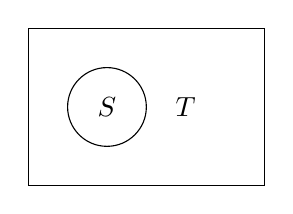
\begin{tikzpicture}
         \draw (0,0) rectangle (3,2);
         \draw (1,1) node {$S$} circle (0.5);
         \draw (2,1) node {$T$};
      \end{tikzpicture}
   \end{center}
   \caption{Region~$S$ is a proper subset of Region~$T$, which completely
   encloses Region~$S$.}
\label{fig:proper-subset}
\end{figure}

\noindent In Figure~\ref{fig:proper-subset}, Region~$S$ inside the circle is
drawn as a proper subset of Region~$T$ inside the rectangle.  Several
properties follow from the definition of subset. The proof of each is left as
an exercise.

\begin{lemma}
   If $A$ and $B$ be sets, and if $A = B$, then $A \subset B$, and $B \subset
   A$.
\label{prop:mutual-subsets}
\end{lemma}

\begin{lemma}
   If $A$ and $B$ be sets such that $A \subset B$, and $B \subset A$, then $A =
   B$.
\end{lemma}

\begin{lemma}
   If $A$, $B$, and $C$ be sets such that $A \subset B$, and $B \subset C$,
   then $A \subset C$.
\end{lemma}

\begin{lemma}
   If $A$ be a set, then $A \subset A$.
\end{lemma}

\noindent Note that although every set $A$ is a subset of itself, $A$ is not a
proper subset of itself.

\subsection{Union}

\begin{definition}
   By ``the union of the sets $S$ and $T$'' we refer to the set whose every
   element is also an element of $S$, of $T$, or else of both $S$ and $T$, and
   we write $S \cup T$.
\end{definition}

\begin{figure}
   \begin{center}
      \begin{tikzpicture}
         \draw (0,0) rectangle (3,2);
         \draw [pattern=north east lines, pattern color=green] (1,1) node {$S$}
         circle (0.75);
         \draw [pattern=north east lines, pattern color=green] (2,1) node {$T$}
         circle (0.75);
         \draw (4,0) rectangle (7,2);
         \draw [pattern=north east lines, pattern color=green] (5,1) node {$S$}
         circle (0.4);
         \draw [pattern=north east lines, pattern color=green] (6,1) node {$T$}
         circle (0.4);
      \end{tikzpicture}
   \end{center}
   \caption{The hatched region of points either in Region~$S$ or in Region~$T$
   (or in both) represents $S \cup T$.}
\label{fig:union}
\end{figure}

\noindent In Figure~\ref{fig:union}, Region~$S$ inside one circle and
Region~$T$ inside another circle might or might not overlap. In either case,
the union $S \cup T$ is indicated by the hatched region, every point of which
is in at least one of $S$ and $T$.

\subsection{Intersection, Empty Set}

\begin{definition}
   By ``the intersection of the sets $S$ and $T$'' we refer to the set whose
   every element is also an element of both $S$ and $T$, and we write $S \cap
   T$.
\end{definition}

\begin{figure}
   \begin{center}
      \begin{tikzpicture}
         \draw (0,0) rectangle (3,2);
         \draw [pattern=north east lines, pattern color=green] (1,1) node {$S$}
         circle (0.75);
         \draw [pattern=north west lines, pattern color=green] (2,1) node {$T$}
         circle (0.75);
         \draw (4,0) rectangle (7,2);
         \draw [pattern=north east lines, pattern color=green] (5,1) node {$S$}
         circle (0.4);
         \draw [pattern=north west lines, pattern color=green] (6,1) node {$T$}
         circle (0.4);
      \end{tikzpicture}
   \end{center}
   \caption{The cross-hatched region in which Region~$S$ overlaps Region~$T$
   represents $S \cap T$. When there be no overlap, $S \cap T = \text{\O}$.}
\label{fig:intersection}
\end{figure}

\noindent In Figure~\ref{fig:intersection}, the case on the left depicts the
situation in which Region~$S$ inside one circle and Region~$T$ inside another
circle overlap. The intersection $S \cap T$ is indicated by the cross-hatched
region, every point of which is in both $S$ and $T$.

\begin{definition}
   By ``the null set'' or ``the empty set'' we refer to the set that has no
   members, and we write \O\ or $\{\}$.
\end{definition}

\noindent It is possible for two sets $S$ and $T$ not to have any elements in
common.  Such a case is depicted in the case on the right in
Figure~\ref{fig:intersection}.  In such a case, $S \cap T = \text{\O}$.  The
null set has the interesting property of being a subset of every set.

\begin{theorem}
   If $A$ be a set, then $\text{\O} \subset A$.
   \begin{proof}
      We must show that for any set $A$, every element of \O\ is an element of
      $A$. Because \O\ has by definition no elements, one might argue that we
      have nothing to do and that $\text{\O} \subset A$ is true simply by
      definition of \O.
      
      There is, however, another approach. One can rephrase the definition of
      the subset: $P \subset Q$ means that for every set $U$ and for every $u
      \in U$, if $u \in P$, then $u \in Q$. By applying modus
      tollens,\footnote{%
         The Latin words ``modus tollens'' mean ``the method of denying''.
         Suppose that if some proposition $S$ be true, then some other
         proposition $T$ must also be true. In that case, whenever $T$ be
         false, then one knows also that $S$ is false. For example, suppose
         that if rain be falling, then there must be a cloud in the sky. If one
         observe that there is not a cloud in the sky, then, if one feel water
         drops falling upon one's skin, one knows that the drops are not drops
         of rain.
      }
      we find the equivalent assertion that if $u \notin Q$, then $u \notin P$.
      So we must show that, for any sets $A$ and $U$, and for every $u \in U$,
      if $u \notin A$ then $u \notin \text{\O}$.  Because, by definition of the
      null set, no element is in \O, every $u$ not in $A$ is also not in \O.
   \end{proof}
\end{theorem}

\subsection{Brace Notation}

A set may be constructed either by listing its elements explicitly or by
referring to a property that every element shares. In either case, curly braces
are used in writing such a construction. An explicit list may be finite or
infinite. For example, $A = \{2, 4, 6\}$ is the set whose members are 2, 4, and
6, and $B = \{2, 4, 6, \ldots\}$ is the set of all positive, even integers. For
an infinite set so constructed, enough of the members must be listed so that
the pattern is clearly evident. An example of construction by property is $C =
\{x \in B: \text{$x$ is a perfect square}\}$; $C$ is then the set containing
only every even number that is a perfect square.

We are now in a position to write a compact expression for each of the union
and the intersecion. If for some set $U$, both $A \subset U$ and $B \subset U$,
then
\begin{eqnarray}
   A \cup B &=& \{x \in U: \text{$x \in A$ or $x \in B$}\}\\
   A \cap B &=& \{x \in U: \text{$x \in A$ and $x \in B$}\}.
\end{eqnarray}

\subsection{Exercises}

\begin{exercise}
   Give three examples of a set. Make sure that each example is not already
   included in the text above.
\end{exercise}
\begin{exercise}
   Let $\mathbb{Z} = \{\ldots, -3, -2, -1, 0, 1, 2, 3, \ldots\}$ be the set of
   all integers. Find a set $A$ and a set $B$ such that $A \subset B \subset
   \mathbb{Z}$.
\end{exercise}
\begin{exercise}
   List the eight subsets of $\{a, b, c\}$.
   \begin{solution}
      Remember that the empty set is a subset of every set and that every set
      is a subset of itself. So the subsets of $\{a,b,c\}$ are $\text{\O},
      \{a\}, \{b\}, \{c\}, \{a, b\}, \{a, c\}, \{b, c\}$, and $\{a, b, c\}$
   \end{solution}
\end{exercise}
\begin{exercise}
   Let $A = \{1, 2, 3, 4, 5\}$, $B = \{2,4\}$, and $C = \{3,5\}$. Find $A \cup
   B$, $(A \cup B) \cup C$, $(B \cup A) \cap C$, $(A \cap B) \cup C$, and $(A
   \cap B) \cap C$.
\end{exercise}
\begin{exercise}
   Prove all of the unproved lemmas in the text above.
\end{exercise}
\begin{exercise}
   Prove that $A \cap B \subset A$ and that $A \subset A \cup B$.
   \begin{solution}
      There are two statements to prove.
      \begin{enumerate}
         \item To prove that $A \cap B \subset A$, we must show that every
            element of $A \cap B$ is an element of $A$. By the definition of
            intersection, every element of $A \cap B$ is both an element of $A$
            and an element of $B$. Therefore, every element of $A \cap B$ is an
            element of $A$.
         \item To prove that $A \subset A \cup B$, we must show that every
            element of $A$ is an element of $A \cup B$. By the definition of
            union, $A \cup B$ contains every element that is either in $A$ or
            in $B$. Therefore, every element of $A$ is an element of $A \cup
            B$.
      \end{enumerate}
   \end{solution}
\end{exercise}

\section{Function}

In the previous section, we explored some possibilities for the relationship
between two sets.  We considered whether an element of one set is also an
element of the other. We defined the subset, the intersection, and the union.

In the present section, we explore some other possibilities. We now consider
pairs of elements. We define terms involved in the consideration of pairs. We
use these terms to talk about a generic \emph{relation} from one set to
another, a specific relation called a \emph{function}, and three subspecies of
function.

\begin{definition}
   An \emph{ordered pair} is a set with two elements along with the ordering
   according to which one of the elements is the \emph{first} element, and the
   other is the \emph{second}. If the first element be $a$ and the second be
   $b$, then we write the ordered pair as $(a,b)$.
\end{definition}

\begin{definition}
   The \emph{Cartesian product} $A \times B$ of any two sets $A$ and $B$ is the
   set of all ordered pairs $(a,b)$, such that $a \in A$ and $b \in B$.
\end{definition}

\noindent For example, if $A = \{1, 2\}$ and $B = \{3, 4, 5\}$, then
\begin{equation*}
   A \times B = \{(1,3), (1,4), (1,5), (2,3), (2,4), (2,5)\}.
\end{equation*}

\subsection{Relation}

\begin{definition}
   A \emph{relation} from a set $A$ to a set $B$ is a subset of $A \times B$.
\end{definition}

\begin{figure}
   \begin{center}
      \begin{minipage}{0.8\columnwidth}
         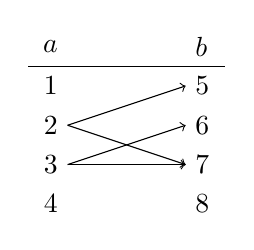
\begin{tikzpicture}[scale=0.5,baseline=(current bounding box.north)]
            \draw (0,+3) node[anchor=east] {$a$};
            \draw (3,+3) node[anchor=west] {$b$};
            \draw (-1,+2.5) -- (4,+2.5);
            \draw (0,+2) node[anchor=east] {$1$};
            \draw (0,+1) node[anchor=east] {$2$};
            \draw (0,+0) node[anchor=east] {$3$};
            \draw (0,-1) node[anchor=east] {$4$};
            \draw (3,+2) node[anchor=west] {$5$};
            \draw (3,+1) node[anchor=west] {$6$};
            \draw (3,+0) node[anchor=west] {$7$};
            \draw (3,-1) node[anchor=west] {$8$};
            \draw[->] (0,+1) -- (3,+2);
            \draw[->] (0,+1) -- (3,+0);
            \draw[->] (0,+0) -- (3,+1);
            \draw[->] (0,+0) -- (3,+0);
         \end{tikzpicture}
         \hfill
         \begin{tikzpicture}[scale=0.5,baseline=(current bounding box.north)]
            \draw[->] (8,0) -- (13,0);
            \draw[->] (8,0) -- (8,5);
            \draw (9,0) node[anchor=north] {1};
            \draw (10,0) node[anchor=north] {2};
            \draw (11,0) node[anchor=north] {3};
            \draw (12,0) node[anchor=north] {4};
            \draw (8,1) node[anchor=east] {5};
            \draw (8,2) node[anchor=east] {6};
            \draw (8,3) node[anchor=east] {7};
            \draw (8,4) node[anchor=east] {8};
            \filldraw (10,1) circle[radius=0.1];
            \filldraw (10,3) circle[radius=0.1];
            \filldraw (11,2) circle[radius=0.1];
            \filldraw (11,3) circle[radius=0.1];
            \draw (10.5,-1.5) node {$a$};
            \draw (6.5,2.5) node {$b$};
         \end{tikzpicture}
      \end{minipage}
   \end{center}
   \caption{Diagram (left) and graph (right) showing a relation from one set,
      whose every element is represented by $a$, to another set, whose every
      element is represented by $b$. In the diagram of a relation, each of zero
      or more elements in the left column may point to zero or more elements in
      the right column. Similarly, in the graph of a relation, each of zero or
      more columns may contain zero or more dots.%
   }
\label{fig:relation}
\end{figure}

\noindent A relation from a set $A$ to a set $B$ is an association between each
of zero or more members of the first set and zero or more members of the second
set.  Suppose that $A = \{1, 2, 3, 4\}$, and $B = \{5, 6, 7, 8\}$. An example
of a relation from $A$ to $B$ is
\begin{equation*}
   R = \{(2,5), (2,7), (3,6), (3,7)\}.
\end{equation*}
Figure~\ref{fig:relation} shows the \emph{diagram} and the \emph{graph} for the
relation. Each of the diagram and the graph expresses the idea of $R$.  In the
diagram, each ordered pair of the relation corresponds to an arrow that points
from a member of $A$ to a member of $B$.  In the graph, each ordered pair of
the relation corresponds to a black dot whose column is given by the first
element of the ordered pair and whose row is given by the second element of the
ordered pair.

\begin{figure}
   \begin{center}
      \begin{minipage}{0.8\columnwidth}
         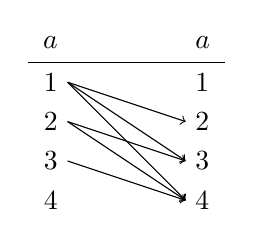
\begin{tikzpicture}[scale=0.5,baseline=(current bounding box.north)]
            \draw (0,+0) node[anchor=east] {$a$};
            \draw (3,+0) node[anchor=west] {$a$};
            \draw (-1,-0.5) -- (4,-0.5);
            \draw (0,-1) node[anchor=east] {$1$};
            \draw (0,-2) node[anchor=east] {$2$};
            \draw (0,-3) node[anchor=east] {$3$};
            \draw (0,-4) node[anchor=east] {$4$};
            \draw (3,-1) node[anchor=west] {$1$};
            \draw (3,-2) node[anchor=west] {$2$};
            \draw (3,-3) node[anchor=west] {$3$};
            \draw (3,-4) node[anchor=west] {$4$};
            \draw[->] (0,-1) -- (3,-2);
            \draw[->] (0,-1) -- (3,-3);
            \draw[->] (0,-1) -- (3,-4);
            \draw[->] (0,-2) -- (3,-3);
            \draw[->] (0,-2) -- (3,-4);
            \draw[->] (0,-3) -- (3,-4);
         \end{tikzpicture}
         \hfill
         \begin{tikzpicture}[scale=0.5,baseline=(current bounding box.north)]
            \draw[->] (0,0) -- (5,0);
            \draw[->] (0,0) -- (0,5);
            \draw (1,0) node[anchor=north] {1};
            \draw (2,0) node[anchor=north] {2};
            \draw (3,0) node[anchor=north] {3};
            \draw (4,0) node[anchor=north] {4};
            \draw (0,1) node[anchor=east] {1};
            \draw (0,2) node[anchor=east] {2};
            \draw (0,3) node[anchor=east] {3};
            \draw (0,4) node[anchor=east] {4};
            \filldraw (1,2) circle[radius=0.1];
            \filldraw (1,3) circle[radius=0.1];
            \filldraw (1,4) circle[radius=0.1];
            \filldraw (2,3) circle[radius=0.1];
            \filldraw (2,4) circle[radius=0.1];
            \filldraw (3,4) circle[radius=0.1];
            \draw (2.5,-1.5) node {$a$};
            \draw (-1.5,2.5) node {$a$};
         \end{tikzpicture}
      \end{minipage}
   \end{center}
   \caption{Diagram (left) and graph (right) of the less-than relation on a
      small set of consecutive integers.%
   }
\label{fig:less-than}
\end{figure}

A relation can also be defined on a single set; that is, from a set to itself.
Consider, as an example of such a relation, the idea given by the words ``less
than'' on the set $A$ in the previous example.  The relation is a subset of $A
\times A$ and can be written as
\begin{equation*}
   R = \{(1,2), (1,3), (1,4), (2,3), (2,4), (3,4)\}.
\end{equation*}
The first element of each ordered pair is less than the second. The diagram and
graph are shown in Figure~\ref{fig:less-than}.  In the diagram, each arrow
expresses the idea that the element at the tail is less than the element at the
head. In the graph, the presence of a dot indicates that the element
corresponding to the dot's column is less than the element corresponding to the
dot's row.

\subsection{Function}

\begin{definition}
   A \emph{function} $f$ is a relation from a set $A$ to a set $B$ such that
   every element of $A$ is associated with exactly one element of $B$. The set
   $A$ is the \emph{domain}, and $B$ is the \emph{co}domain. For every $a \in
   A$, the corresponding element in $B$ is written $f(a)$.
\end{definition}

\begin{figure}
   \begin{center}
      \begin{minipage}{0.8\columnwidth}
         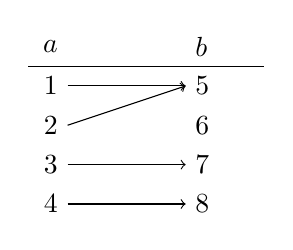
\begin{tikzpicture}[scale=0.5,baseline=(current bounding box.north)]
            \draw (0,+0) node[anchor=east] {$a$};
            \draw (3,+0) node[anchor=west] {$b$};
            \draw (-1,-0.5) -- (5,-0.5);
            \draw (0,-1) node[anchor=east] {$1$};
            \draw (0,-2) node[anchor=east] {$2$};
            \draw (0,-3) node[anchor=east] {$3$};
            \draw (0,-4) node[anchor=east] {$4$};
            \draw (3,-1) node[anchor=west] {$5$};
            \draw (3,-2) node[anchor=west] {$6$};
            \draw (3,-3) node[anchor=west] {$7$};
            \draw (3,-4) node[anchor=west] {$8$};
            \draw[->] (0,-1) -- (3,-1);
            \draw[->] (0,-2) -- (3,-1);
            \draw[->] (0,-3) -- (3,-3);
            \draw[->] (0,-4) -- (3,-4);
         \end{tikzpicture}
         \hfill
         \begin{tikzpicture}[scale=0.5,baseline=(current bounding box.north)]
            \draw[->] (0,0) -- (5,0);
            \draw[->] (0,0) -- (0,5);
            \draw (1,0) node[anchor=north] {1};
            \draw (2,0) node[anchor=north] {2};
            \draw (3,0) node[anchor=north] {3};
            \draw (4,0) node[anchor=north] {4};
            \draw (0,1) node[anchor=east] {5};
            \draw (0,2) node[anchor=east] {6};
            \draw (0,3) node[anchor=east] {7};
            \draw (0,4) node[anchor=east] {8};
            \filldraw (1,1) circle[radius=0.1];
            \filldraw (2,1) circle[radius=0.1];
            \filldraw (3,3) circle[radius=0.1];
            \filldraw (4,4) circle[radius=0.1];
            \draw (2.5,-1.5) node {$a$};
            \draw (-1.75,2.5) node {$b$};
         \end{tikzpicture}
      \end{minipage}
   \end{center}
   \caption{Function from a domain, whose every element is represented by $a$,
      to a codomain, whose every element is represented by $b$. In the diagram
      of a function, every element in the left column points to exactly one
      element in the right column. Similarly, in the graph of a function, every
      column contains exactly one dot.%
   }
\label{fig:function}
\end{figure}

\noindent A mere relation from $A$ to $B$ might associate more than one element
of $B$ with an element of $A$, and it might not make an association for every
element of $A$. A function, however, associates every element of $A$ with
exactly one element of $B$, though not every element of $B$ need have an
association, and an element of $B$ might be associated with more than one
element of $A$. Suppose that $A = \{1, 2, 3, 4\}$, and $B = \{5, 6, 7, 8\}$.
An example of a function from $A$ to $B$ is
\begin{equation*}
   f = \{(1,5), (2,5), (3,7), (4,8)\}.
\end{equation*}
The diagram and graph for $f$ are shown in Figure~\ref{fig:function}.  In the
diagram, every element of $A$ lies at the tail of an arrow, and no more than
one arrow originates at an element of $A$.  In the graph, there is a dot for
every element of $A$ (for every column), and no column contains more than one
dot.  This is characteristic of a function.

A function may be defined by specifying a single rule that operates on every
member of the domain. For example $f(x) = x^2$ defines a function that maps
every element of the domain to the element's square.

\subsection{Injection}

\begin{definition}
   An \emph{injection}\footnote{%
      By its etymology, ``injection'' indicates that which is thrown into
      something else. The word is used to name a function that might not map
      its domain completely to cover the codomain (so the domain is thrown
      somewhere inside the codomain) but does make sure that every element of
      the domain does map to its own element of the codomain.
   }
   $f$ from a set $A$ to a set $B$ is a function such that, for every $a_1 \in
   A$ and $a_2 \in A$, if $a_1 \neq a_2$, then $f(a_1) \neq f(a_2)$. An
   injection maps from its domain to its codomain in a \emph{one-to-one} way;
   so an injection is sometimes called a ``one-to-one function''.
\end{definition}

\begin{figure}
   \begin{center}
      \begin{minipage}{0.8\columnwidth}
         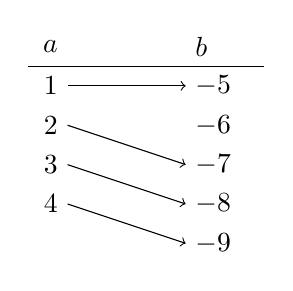
\begin{tikzpicture}[scale=0.5,baseline=(current bounding box.north)]
            \draw (0,+0) node[anchor=east] {$a$};
            \draw (3,+0) node[anchor=west] {$b$};
            \draw (-1,-0.5) -- (5,-0.5);
            \draw (0,-1) node[anchor=east] {$1$};
            \draw (0,-2) node[anchor=east] {$2$};
            \draw (0,-3) node[anchor=east] {$3$};
            \draw (0,-4) node[anchor=east] {$4$};
            \draw (3,-1) node[anchor=west] {$-5$};
            \draw (3,-2) node[anchor=west] {$-6$};
            \draw (3,-3) node[anchor=west] {$-7$};
            \draw (3,-4) node[anchor=west] {$-8$};
            \draw (3,-5) node[anchor=west] {$-9$};
            \draw[->] (0,-1) -- (3,-1);
            \draw[->] (0,-2) -- (3,-3);
            \draw[->] (0,-3) -- (3,-4);
            \draw[->] (0,-4) -- (3,-5);
         \end{tikzpicture}
         \hfill
         \begin{tikzpicture}[scale=0.5,baseline=(current bounding box.north)]
            \draw[->] (0,0) -- (5,0);
            \draw[->] (0,0) -- (0,6);
            \draw (1,0) node[anchor=north] {$1$};
            \draw (2,0) node[anchor=north] {$2$};
            \draw (3,0) node[anchor=north] {$3$};
            \draw (4,0) node[anchor=north] {$4$};
            \draw (0,1) node[anchor=east] {$-5$};
            \draw (0,2) node[anchor=east] {$-6$};
            \draw (0,3) node[anchor=east] {$-7$};
            \draw (0,4) node[anchor=east] {$-8$};
            \draw (0,5) node[anchor=east] {$-9$};
            \filldraw (1,1) circle[radius=0.1];
            \filldraw (2,3) circle[radius=0.1];
            \filldraw (3,4) circle[radius=0.1];
            \filldraw (4,5) circle[radius=0.1];
            \draw (2.5,-1.5) node {$a$};
            \draw (-2.25,3) node {$b$};
         \end{tikzpicture}
      \end{minipage}
   \end{center}
   \caption{Injection. In the diagram of an injective function, every element
      in the right column is pointed to by no more than one element in the left
      column. Similarly, in the graph of an injective function, every row
      contains no more than one dot.%
   }
\label{fig:injection}
\end{figure}

\noindent Suppose that $A = \{1, 2, 3, 4\}$, and $B = \{-5, -6, -7, -8, -9\}$.
An example of an injection from $A$ to $B$ is
\begin{equation*}
   f = \{(1,-5), (2,-7), (3,-8), (4,-9)\}.
\end{equation*}
The diagram and graph for $f$ are shown in Figure~\ref{fig:injection}.  In the
diagram, no more than one arrow terminates at any single element of $B$.  In
the graph, no row contains more than one dot.  This is characteristic of an
injection.

\subsection{Surjection}

\begin{definition}
   A \emph{surjection}\footnote{%
      In coming to us from Latin through French, the prefix ``super'' changed
      to ``sur''. By its etymology, ``surjection'' indicates that which is
      thrown over or on top of something else. The word is used to name a
      function that throws its domain on top of its codomain so that the
      codomain is completely covered by the domain.
   }
   $f$ from a set $A$ to a set $B$ is a function such that, for every element
   $b \in B$, there is at least one element $a \in A$ for which $b = f(a)$. A
   surjection maps its domain \emph{onto} its codomain; so a surjection is
   sometimes called an ``onto function''.
\end{definition}

\begin{figure}
   \begin{center}
      \begin{minipage}{0.8\columnwidth}
         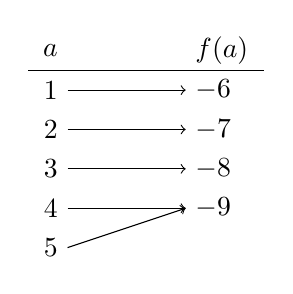
\begin{tikzpicture}[scale=0.5,baseline=(current bounding box.north)]
            \draw (0,+0) node[anchor=east] {$a$};
            \draw (3,+0) node[anchor=west] {$f(a)$};
            \draw (-1,-0.5) -- (5,-0.5);
            \draw (0,-1) node[anchor=east] {$1$};
            \draw (0,-2) node[anchor=east] {$2$};
            \draw (0,-3) node[anchor=east] {$3$};
            \draw (0,-4) node[anchor=east] {$4$};
            \draw (0,-5) node[anchor=east] {$5$};
            \draw (3,-1) node[anchor=west] {$-6$};
            \draw (3,-2) node[anchor=west] {$-7$};
            \draw (3,-3) node[anchor=west] {$-8$};
            \draw (3,-4) node[anchor=west] {$-9$};
            \draw[->] (0,-1) -- (3,-1);
            \draw[->] (0,-2) -- (3,-2);
            \draw[->] (0,-3) -- (3,-3);
            \draw[->] (0,-4) -- (3,-4);
            \draw[->] (0,-5) -- (3,-4);
         \end{tikzpicture}
         \hfill
         \begin{tikzpicture}[scale=0.5,baseline=(current bounding box.north)]
            \draw[->] (0,0) -- (6,0);
            \draw[->] (0,0) -- (0,5);
            \draw (1,0) node[anchor=north] {$1$};
            \draw (2,0) node[anchor=north] {$2$};
            \draw (3,0) node[anchor=north] {$3$};
            \draw (4,0) node[anchor=north] {$4$};
            \draw (5,0) node[anchor=north] {$5$};
            \draw (0,1) node[anchor=east] {$-6$};
            \draw (0,2) node[anchor=east] {$-7$};
            \draw (0,3) node[anchor=east] {$-8$};
            \draw (0,4) node[anchor=east] {$-9$};
            \filldraw (1,1) circle[radius=0.1];
            \filldraw (2,2) circle[radius=0.1];
            \filldraw (3,3) circle[radius=0.1];
            \filldraw (4,4) circle[radius=0.1];
            \filldraw (5,4) circle[radius=0.1];
            \draw (3,-1.5) node {$a$};
            \draw (-2.25,2.5) node {$f(a)$};
         \end{tikzpicture}
      \end{minipage}
   \end{center}
   \caption{Surjection. In the diagram of a surjective function, every element
      in the right column is pointed to by at least one element in the left
      column. Similarly, in the graph of a surjective function, every row
      contains at least one dot.%
   }
\label{fig:surjection}
\end{figure}

\noindent Suppose that $A = \{1, 2, 3, 4, 5\}$, and $B = \{-6, -7, -8, -9\}$.
An example of an surjection from $A$ to $B$ is
\begin{equation*}
   f = \{(1,-6), (2,-7), (3,-8), (4,-9), (5,-9)\}.
\end{equation*}
For every element $b \in B$, there is at least one $a \in A$ such that $b =
f(a)$.  So, for a surjection, the diagram and graph may refer to $f(a)$ rather
than to $b$. The diagram and graph for $f$ are shown in
Figure~\ref{fig:surjection}.  In the diagram, every element of $B$ has at least
one arrow terminating on the element. In the graph, every row contains at least
one dot.  This is characteristic of a surjection.

\begin{definition}
   For any function $f$, the \emph{image} of its domain $A$ is the set $\{f(a)
   : a \in A\}$.
\end{definition}

\noindent By this definition, a surjection is just a function whose codomain is
equal to the image of the domain.

\subsection{Bijection}

\begin{definition}
   A \emph{bijection} $f$ from a set $A$ to a set $B$ is both an injection and
   a surjection.
\end{definition}

\begin{figure}
   \begin{center}
      \begin{minipage}{0.8\columnwidth}
         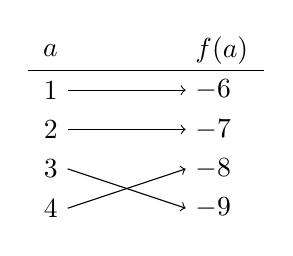
\begin{tikzpicture}[scale=0.5,baseline=(current bounding box.north)]
            \draw (0,+0) node[anchor=east] {$a$};
            \draw (3,+0) node[anchor=west] {$f(a)$};
            \draw (-1,-0.5) -- (5,-0.5);
            \draw (0,-1) node[anchor=east] {$1$};
            \draw (0,-2) node[anchor=east] {$2$};
            \draw (0,-3) node[anchor=east] {$3$};
            \draw (0,-4) node[anchor=east] {$4$};
            \draw (3,-1) node[anchor=west] {$-6$};
            \draw (3,-2) node[anchor=west] {$-7$};
            \draw (3,-3) node[anchor=west] {$-8$};
            \draw (3,-4) node[anchor=west] {$-9$};
            \draw[->] (0,-1) -- (3,-1);
            \draw[->] (0,-2) -- (3,-2);
            \draw[->] (0,-3) -- (3,-4);
            \draw[->] (0,-4) -- (3,-3);
         \end{tikzpicture}
         \hfill
         \begin{tikzpicture}[scale=0.5,baseline=(current bounding box.north)]
            \draw[->] (0,0) -- (6,0);
            \draw[->] (0,0) -- (0,5);
            \draw (1,0) node[anchor=north] {$1$};
            \draw (2,0) node[anchor=north] {$2$};
            \draw (3,0) node[anchor=north] {$3$};
            \draw (4,0) node[anchor=north] {$4$};
            \draw (0,1) node[anchor=east] {$-6$};
            \draw (0,2) node[anchor=east] {$-7$};
            \draw (0,3) node[anchor=east] {$-8$};
            \draw (0,4) node[anchor=east] {$-9$};
            \filldraw (1,1) circle[radius=0.1];
            \filldraw (2,2) circle[radius=0.1];
            \filldraw (3,4) circle[radius=0.1];
            \filldraw (4,3) circle[radius=0.1];
            \draw (2.5,-1.5) node {$a$};
            \draw (-2.25,2.5) node {$f(a)$};
         \end{tikzpicture}
      \end{minipage}
   \end{center}
   \caption{Bijection. In the diagram of a bijective function, every element in
      the right column is pointed to by exactly one element in the left column.
      Similarly, in the graph of a bijective function, every row contains
      exactly one dot.%
   }
\label{fig:bijection}
\end{figure}

\noindent Suppose that $A = \{1, 2, 3, 4\}$, and $B = \{-6, -7, -8, -9\}$.  An
example of an bijection from $A$ to $B$ is
\begin{equation*}
   f = \{(1,-6), (2,-7), (3,-9), (4,-8)\}.
\end{equation*}
For every element $b \in B$, there is exactly one $a \in A$ such that $b =
f(a)$. The diagram and graph for $f$ are shown in Figure~\ref{fig:bijection}.
In the diagram, every element of $B$ has exactly one arrow terminating on the
element.  In the graph of $f$, every row has exactly one dot in it.  This is
characteristic of a bijection.  A bijection both
\begin{itemize}
   \item pairs every element of the domain with exactly one element of the
      codomain and
   \item pairs every element of the codomain with exactly one element of the
      domain.
\end{itemize}

\begin{theorem}
   For every bijection $f$ from a set $A$ to a set $B$, there is an inverse
   function $g$ from $B$ to $A$ such that for every $b \in B$, $f(g(b)) = b$,
   and for every $a \in A$, $g(f(a)) = a$.
\label{theorem:func-inverse}
\end{theorem}

\begin{definition}
   For a bijection $f$, its inverse is written $f^{-1}$.
\end{definition}

\subsection{Exercises}

\begin{exercise}
   Let $A = \{0,2,4\}$ and $B = \{1,3,5\}$. What is $A \times B$?
\end{exercise}

\begin{exercise}
   Pick a set of six numbers, and define on the set the relation expressing the
   idea given by the words ``greater than''. List the elements of the relation;
   draw the diagram of the relation; and draw the graph of the relation.
\end{exercise}

\begin{exercise}
   Pick a set of six numbers, and define a function from the set to itself.
   List the elements of the function; draw the diagram of the function; and
   draw the graph of the function.
\end{exercise}

\begin{exercise}
   Pick a set of six numbers, and define an injection from the set to itself.
   List the elements of the function; draw the diagram of the function; and
   draw the graph of the function.
\end{exercise}

\begin{exercise}
   Pick a set of six numbers, and define a surjection from the set to itself
   such that the function is also an injection.  List the elements of the
   function; draw the diagram of the function; and draw the graph of the
   function.
\end{exercise}

\begin{exercise}
   Pick a set of six numbers, and define a surjection from the set to itself
   such that the function is not also an injection.  List the elements of the
   function; draw the diagram of the function; and draw the graph of the
   function.
\end{exercise}

\begin{exercise}
   Pick two sets of numbers, and define an injection from one set to the other
   such that the function is not also a surjection.  List the elements of the
   function; draw the diagram of the function; and draw the graph of the
   function.
\end{exercise}

\begin{exercise}
   Prove Theorem~\ref{theorem:func-inverse}. Hint: Remember that a bijection
   $f$ from a set $A$ to a set $B$ is a kind of function, which is a kind of
   relation, which is a subset of $A \times B$. Consider the elements of $f$.
   Each element is an ordered pair. Now consider from $B \times A$ the subset
   $g$ that is obtained by reversing the order of every element of $f$. Show
   that the elements of $g$ behave exactly as they would if $g = f^{-1}$.
\end{exercise}

